\documentclass[border=4pt]{standalone}
% Shared style for every diagram. Colour-blind-safe palette (Okabe-Ito).
\usepackage[T1]{fontenc}
\usepackage{helvet}
\renewcommand{\familydefault}{\sfdefault}
\usepackage{tikz}
\usetikzlibrary{arrows.meta,positioning,fit,backgrounds,calc,shapes.geometric,decorations.pathreplacing}
\definecolor{cblue}{HTML}{0072B2}
\definecolor{corange}{HTML}{E69F00}
\definecolor{cgreen}{HTML}{009E73}
\definecolor{cred}{HTML}{D55E00}
\definecolor{cpurple}{HTML}{CC79A7}
\definecolor{cgrey}{HTML}{6B7280}
\definecolor{csky}{HTML}{56B4E9}
\tikzset{
  >={Stealth[length=2.2mm]},
  box/.style={draw, rounded corners=3pt, align=center, minimum height=11mm, minimum width=22mm, font=\small, line width=0.7pt},
  real/.style={box, draw=cblue, fill=cblue!8},
  sim/.style={box, draw=corange, fill=corange!12},
  future/.style={box, draw=cgrey, dashed, fill=white},
  flow/.style={->, line width=0.8pt, draw=black!75},
  dflow/.style={->, line width=0.8pt, dashed, draw=cgrey},
  lbl/.style={font=\scriptsize, text=black!70},
  group/.style={draw=black!25, rounded corners=6pt, inner sep=6pt},
}

\begin{document}
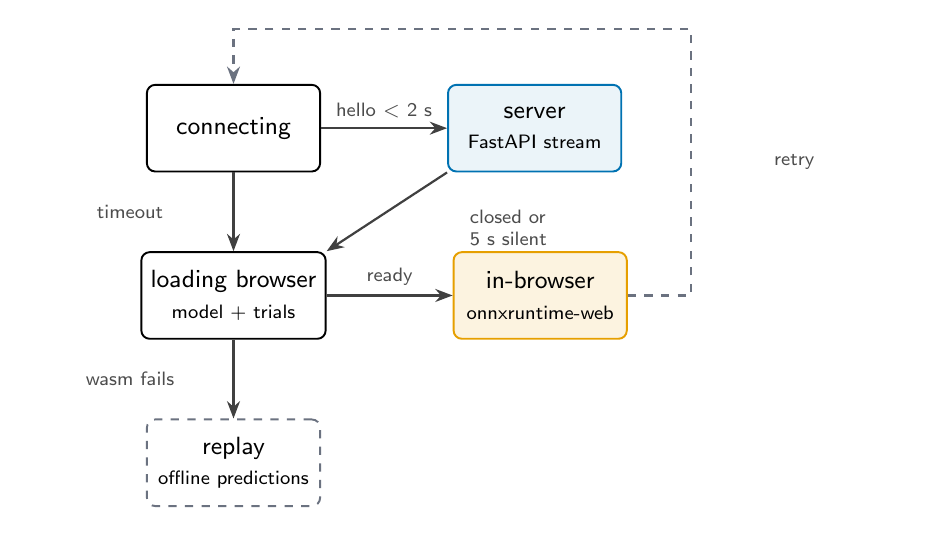
\begin{tikzpicture}[node distance=10mm and 16mm, every node/.append style={minimum width=26mm}]
  \node[box] (conn) {connecting};
  \node[real, right=of conn] (srv) {server\\\scriptsize FastAPI stream};
  \node[box, below=of conn] (load) {loading browser\\\scriptsize model + trials};
  \node[sim, right=of load] (br) {in-browser\\\scriptsize onnxruntime-web};
  \node[future, below=of load] (rep) {replay\\\scriptsize offline predictions};
  \draw[flow] (conn) -- node[lbl, above] {hello $<$ 2 s} (srv);
  \draw[flow] (conn) -- node[lbl, left] {timeout} (load);
  \draw[flow] (srv.south west) -- node[lbl, pos=0.35, below right, align=left] {closed or\\5 s silent} (load.north east);
  \draw[flow] (load) -- node[lbl, above] {ready} (br);
  \draw[flow] (load) -- node[lbl, left] {wasm fails} (rep);
  \draw[dflow] (br.east) -- ++(8mm,0) |- node[lbl, pos=0.25, right] {retry} ($(conn.north)+(0,7mm)$) -- (conn.north);
\end{tikzpicture}
\end{document}
